\section{Tests}
\label{TestsSection}
In this section we will describe what tests we have run on the algorithms, and what we expect to see from them.
Section~\ref{AlgCorrectness} contains a brief explanation of the verification we do to ensure that the max flow value returned by our algorithm implementations is the correct one.
Section~\ref{GraphGenerators} contain a list of the different types of graphs we will be running on.


\subsection{Algorithm Correctness}
\label{AlgCorrectness}
To verify that our algorithms work, we use the method of certifying algorithms \cite{McConnell10certifyingalgorithms}.
We implement our algorithms to return both the value of the max flow, and the residual network after all flow has been sent from $s$ to $t$.
We implemented a verifier that runs after the algorithms. It uses the residual network in combination with the original graph to calculate the flow on each edge in the graph.
It then verifies that the value of the max flow returned by the algorithm is the same as both the flow going out of $s$ and the flow going into $t$.
Additionally, it verifies that the excess in all nodes apart from $s$ and $t$ are $0$, and that there are no edges where more flow is sent than what is allowed by the capacity on the edge in the original graph.
By this, we have ensured that the capacity and flow constraints are fulfilled. The last check we do is to make sure that no more flow can be sent from $s$ to $t$. This is done by looking for an augmenting path.

With these checks, we have proof that the max flow returned by the algorithms is the correct ones.
    
\subsection{Graph Generators}
\label{GraphGenerators}
We have various different algorithms to generate different types of graphs to test on.
The graph generation algorithms described in the next Sections are a mix of custom algorithms, and algorithms taken from from DIMACS \cite{Johnson:1993:NFM:562474}.

\subsection{Connected Randomized}
\label{ACGraphsSection}
The AC graph generator from DIMACS produces an acyclic graph with nodes $v_0, \cdots, v_{n-1}$. A node $v_i$ has edges to all nodes $v_{i+1}, \cdots, v_{n-1}$ 
with capacities randomly generated in the range $[1, 10000]$.

The purpose of this generator is to get examples of fully connected graphs where $m$ is close to $n^2$.

When we ran the push-relabel algorithms on this type of graph we got big jumps in the time spent due to the random capacities. 
If everything sent out of source can be sent to the target, the algorithms won't have to relabel all the nodes very far.
On the other hand, if not everything can be sent to the target, it is likely that all nodes will have to be relabelled to $n+1$, since the graph is fully connected.

To get a better picture, we split the AC graphs up into two groups. An easy group where everything can be sent to the target, and a hard group where some of the flow will have to be pushed back.
In these graphs, we connected all nodes except $s$ and $t$, so the graph is cyclic. Capacities on edges from $s$ and edges to $t$ are random in the range $[1, 10000]$. 
All other edges have capacity $10000$ to allow all flow to be sent from one node to the other.

We will abbreviate these types of graphs with CRE and CRH for Connected graphs, Randomized capacities, Easy/Hard for push relabel. 

\begin{figure}[!ht]
\centering
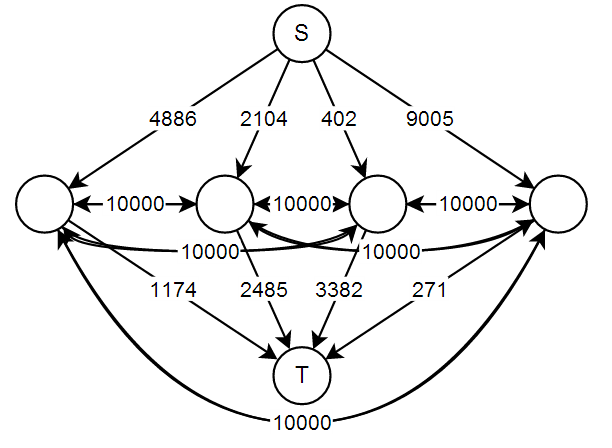
\includegraphics[width=70mm]{CRexample.PNG}
\caption{An example of a CRH graph.}
\label{crh example}
\end{figure}


\subsection{Connected Deterministic}
\label{CDGraphsSection}
We observed very good results for the implementation of the Dinic algorithm in the CRH and CRE graphs.
This is because there are a small number of augmenting paths, and all of those paths have length 2 or 3.

To alleviate this, we made a new type of fully connected graph. 
This graph is designed to contain as many augmenting paths as we could get in there.
We had hoped to get $\Omega(nm)$ augmenting paths to reach the worst case running time for Dinic, but the analysis in the end of this section shows that there are $O(m\log n)$ augmenting paths.
This should make the graph very difficult for augmenting path algorithms like the algorithm by Edmonds and Karp and the algorithm by Dinic.

The graph generator is deterministic for a specific size, and is constructed so that it considers layer graphs of increasing length. An example of how the graph is constructed can be seen in Figure~\ref{badDinicExample}.

\begin{figure}[!ht]
\centering
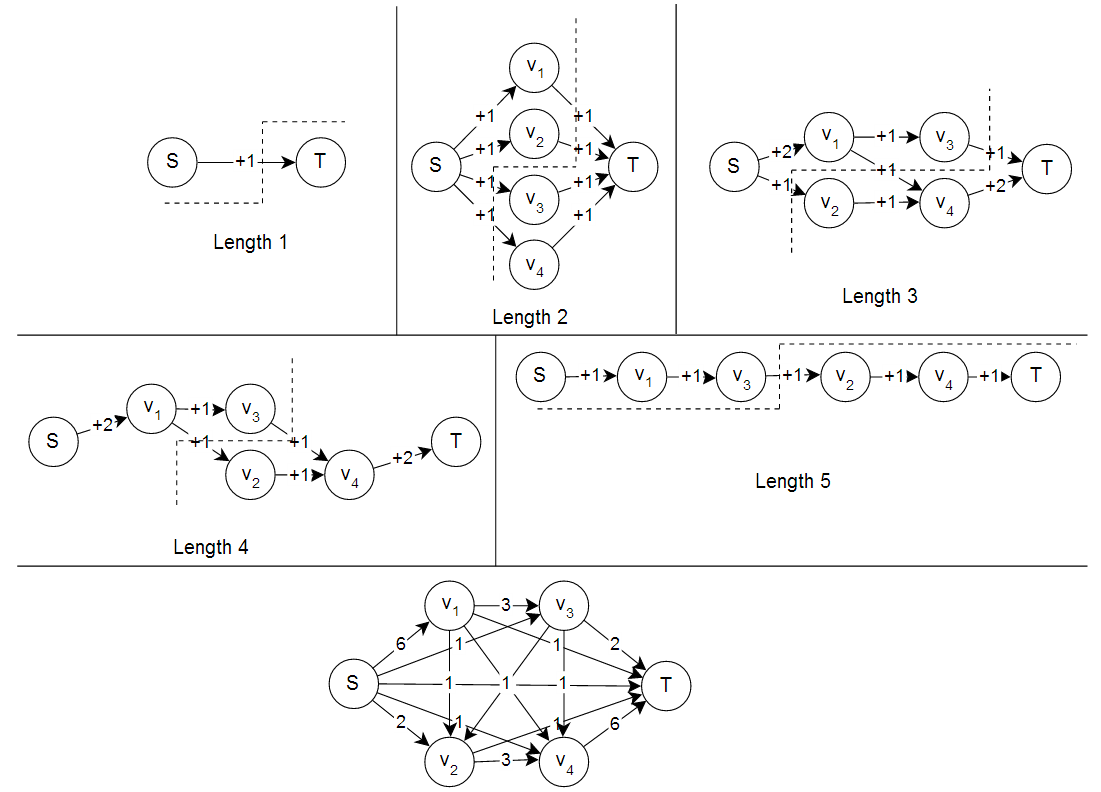
\includegraphics[width=120mm]{BadDinicExample.png}
\caption{How the custom connected graph is constructed for $n=6$.}
\label{badDinicExample}
\end{figure}

The nodes in each layer graph is partitioned into a top half and a bottom half set. The goal is to have the min cut of each layer graph between the top and bottom half sets, so that the bottom half can be offset to the next column in the following layer graph.
The edges going internally in the top or bottom sets just has enough capacity to route the flow that is sent over the cut. 

This allows for nodes to be in different sets in different layer graphs. For example, picture the construction of $n=18$. 
In that construction, $v_{11}$ would go from being in the bottom set in the layer of length $2$ to the top set in layer $3$ and $4$, to the bottom set in layers $5$ to $8$, and then in the top set in layers $9$ to $17$.

Note that for $n \geq 18$, the situation arises where flow will have to be sent from $v_i$ to $v_j$, and in a later layer graph, from $v_j$ to $v_i$.
In that situation, we do not increase the capacity of $(v_j, v_i)$, since it will already have the required residual capacity.
For instance, for $n=18$, in layer $4$, $(v_{11}, v_{14})$ is part of the cut. In layer $8$, $(v_{14}, v_{11})$ is in a cut, and in layer $12$, $(v_{11}, v_{14})$ is back in the cut.

The way the bottom half set is offset ensures that once an edge $(v_i, v_j)$ has been part of a cut, $v_i$ and $v_j$ can not be neighbours in one set, because $v_j$ will be moved to a column at least two columns in front of $v_i$.
So, the only way $(v_i, v_j)$ can be used again is if $(v_i, v_j)$ is part of a future cut. 
In order for that to happen, $v_i$ first has to be moved in front of $v_j$ though, and in order for that to happen, $v_j$ must be in the top set, and $v_i$ in the bottom set.
At that point, $(v_j, v_i)$ would be part of of the cut, meaning that the residual capacity of $(v_i, v_j)$ would return to one, and we can use it again in a cut without increasing its capacity.
This means that once an edge has been part of a cut, its capacity will never increase, so capacity increases won't interfere with the capacity of a cut in a previous layer graphs.

Once two nodes have been placed in the same row, they will be in the same row for the rest of the layers. This means that the edge between them will never be part of the min cut in the future.
For this reason, when flow is routed inside the top or bottom set, it is just sent to the next node in the same row. This ensures that routing flow inside the sets does not interfere with future cuts.

There is one problem in the construction of this graph that we have not been able to eliminate. It is possible for the max flow algorithm to route flow inside a set across rows, because such an edge could be part of a future cut.
Doing this will create an augmenting path in the next layer graph where the edge can be taken the opposite way, so it does not change the number of augmenting paths. However, it does mean that the execution of Dinic does not always find the expected layer graphs.

This construction results in a graph with $m=\frac{n(n-1)}{2}$ non-zero edges. If you also count zero capacity edges $(v_j, v_i)$ that are added as a result of $(v_i, v_j)$ being added, this type of graph contains all edges possible.

The abbreviation for this type of graphs will be CD for Connected graphs, fully Deterministic construction.

To calculate the number of augmenting paths in a graph like this, we consider a different type of graph that has more paths, but is harder to construct in practise.
If we consider a layer graph of length $k$, we can partition the nodes into sets such that $V_i = \{ v\in V \mid distance(s, v) = i\}$.
Every node in $v\in V_i$ will then have an edge from at least one node in $V_{i-1}$, 
but it is not possible for them to have any edges from nodes in $V_j$ where $j<i-1$, since that would place $v$ in $V_{j+1}$. 
If all of edges to a node $v\in V_i$ from nodes in $V_{i-1}$ are saturated as a part of finding the blocking flow, 
$v$ will be promoted to a set $V_j$ where $i<j$ in the next layer graph.
The maximum number of unique paths from $s$ to $t$ in a layer graph of length $k$ is $\prod_{i=1}^{k-1}{|V_i|}$, 
which is the case when all nodes in $V_i$ has an edge to every node in $V_{i+1}$.
This product is maximized when $|V_i|=\frac{n}{k}$, meaning that all sets have the same size. 
Our CD graph is not perfectly rectangular in every layer graph, which is why it has fewer unique paths.

A layer graph could be constructed such that you saturate every edge from $V_i$ to $V_{i+1}$ when finding the blocking flow.
This could lead to $O(n^2)$ edges being saturated, but it would also mean that no more paths can be found from $s$ to $t$ 
since all nodes in $V_{i+1}$ would have been promoted to $V_{i+2}$, and no edges can exist from $V_i$ or less to $V_{i+2}$.
The worst case scenario is if as many edges are saturated as possible, such that the size of all the sets go from $\frac{n}{k}$ to $\frac{n}{k+1}$ in the next layer graph.
To do this, $\frac{i}{k+1}\frac{n}{k}$ nodes have to be promoted from $V_i$ to $V_{i+1}$.
We let $p(i, k)$ and $s(i, k)$ denote the number of nodes that has to be promoted from set $i$ in the layer graph of length $k$, and the number of nodes that stay respectively.
\begin{align*}
p(i, k) &= \frac{i}{k+1}\frac{n}{k}\\
s(i, k) &= \left(1 - \frac{i}{k+1}\right)\frac{n}{k}\\
 &= \frac{k+1-i}{k+1}\frac{n}{k}
\end{align*}
With this, we can verify that all $V_i$ contains $\frac{n}{k+1}$ nodes after going from the layer graph of size $k$ to $k+1$.
\begin{align*}
|V_i|&=s(i, k)+p(i-1, k)\\
&=\frac{k+1-i}{k+1}\frac{n}{k}+\frac{i-1}{k+1}\frac{n}{k}\\
&=\frac{k}{k+1}\frac{n}{k}\\
&=\frac{n}{k+1}
\end{align*}
When going from a layer graph of length $k$ to $k+1$, we are allowed to saturate edges from each node that stays in $V_i$ to nodes in $V_{i+1}$ that are promoted.
That means we can have at most $s(i, k)p(i+1, k)$ edges that are saturated between two sets, and by extension at most $p(1, k)+s(k, k)+\sum_{i=1}^{k-1}{s(i, k)p(i+1, k)}$ 
augmenting paths in the layer graph of length $k$. In that expression, $p(1, k)$ corresponds to edges from $s$ to nodes in $V_1$ that are promoted, 
and $s(k, k)$ corresponds to edges to $t$ from nodes in $V_k$ that are not promoted.
To get the number of augmenting paths in all layer graphs, we sum $k$ from $1$ to $n$.
\begin{align*}
Paths&=\sum_{k=1}^{n}{p(1, k)+s(k, k)+\sum_{i=1}^{k-1}{s(i, k)p(i+1, k)}}\\
&=\sum_{k=1}^{n}{\frac{1}{k+1}\frac{n}{k}+\frac{k+1-k}{k+1}\frac{n}{k}+\sum_{i=1}^{k-1}{\frac{k+1-i}{k+1}\frac{n}{k}\frac{i+1}{k+1}\frac{n}{k}}}\\
&=n\sum_{k=1}^{n}{\frac{2}{k(k+1)}+n\sum_{i=1}^{k-1}{\frac{(k+1-i)(i+1)}{k^2(k+1)^2}}}\\
&\leq n\sum_{k=1}^{n}{\frac{2}{k(k+1)}+n(k-1)\frac{(k+1-k/2)(k/2+1)}{k^2(k+1)^2}}\\
&=n\sum_{k=1}^{n}{\frac{2}{k(k+1)}+n(k-1)\frac{(k+2)^2}{4k^2(k+1)^2}}\\
&=O\left( n\sum_{k=1}^{n}{\frac{2}{k(k+1)}+\frac{n}{k}}\right)\\
&=O\left( n^2\sum_{k=1}^{n}{\frac{1}{k}}\right)\\
&= O\left(n^2\log n\right)
\end{align*}
Note that $(k+1-i)(i+1)=-i^2+ki+(k+1)$ quadratic function $ai^2+bi+c$ with optimum in $i=-\frac{b}{2a}=\frac{k}{2}$. 
That is how the inner sum is removed.

Since our graph is fully connected, this is equal to $O(m\log n)$.
What this means is that CD will not match the worst case bound of Dinic. 
The worst case bound of $O(n^2m)$ came from a bound of $O(m)$ paths per layer graph, $O(n)$ layer graphs, and $k$ time to send flow on a path of length $k$ where $k=O(n)$.
So, on this graph, we would expect Dinic to run in $O(nm\log n)$.
We were not able to come up with a graph with $O(nm)$ augmenting paths, and it is possible that no such graph exists.
If no such graphs exist for any $m$, it could be used as an improved analysis of the Edmonds and Karp, and Dinic algorithms. 

\subsection{AK}
\label{AKGraphSection}
The AK graph generator takes a parameter $k$, and produces deterministic graphs where $n=4k+6$ and $m=6k+7$. 
These graphs are designed to be very hard instances of the max flow problem.

\begin{figure}[!ht]
\centering
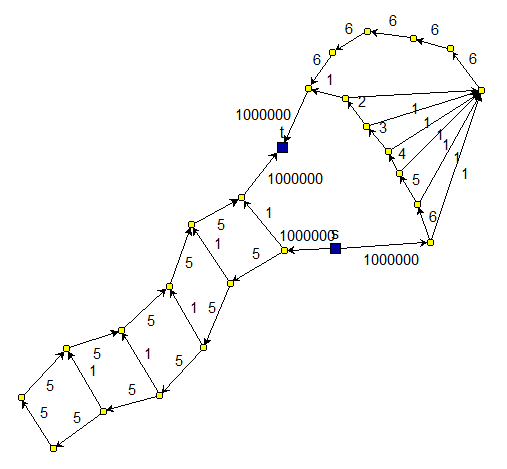
\includegraphics[width=50mm]{ak.png}
\caption{An example of the output of the AK generator, where $n=26$.}
\label{akExample}
\end{figure}

As can be seen in Figure~\ref{akExample}, this type of graphs contain two hard patterns. The left pattern require that the flow is pushed far out in the graph, and then back.
For Push Relabel algorithms, this means that flow will be pushed back and forth in the graph while relabelling. 

With the first global relabel heuristic, a lot of global relabels will occur due to the left pattern, even though flow is not sent around in a cycle. 
This is the reason we decided to implement a second global relabelling heuristic.

The right pattern contains very long paths of increasing length. This is particularly hard for the Dinic algorithm, since will get layer graphs with only one or two augmenting paths.
It is also a place where the algorithms should benefit from dynamic trees, because you can send flow over the long path in $O(\log{k})$ time instead of $O(k)$ time.


\subsection{GenRmf}
\label{GENRMFGraphSection}
The previous graphs are designed to be very hard or very easy for some of the algorithms. The last two types of graphs will be more randomized, to better illustrate typical performance.

The GenRmf generator produces a special kind of graphs developed by Goldfarb and Grigoriads \cite{goldfarb1987computational}.
It takes parameters $a$, $b$, $c_{min}$ and $c_{max}$. The graph produced will consist of $b$ layers of nodes, with $a \times a$ nodes laid out in a square grid in each layer.
Each node in a layer has an edge connecting it to the two to four nodes adjacent to it, as well as a single edge to a random node in the next layer.
The source node is placed in the first layer, and the target node is placed in the last layer.

\begin{figure}[!ht]
\centering
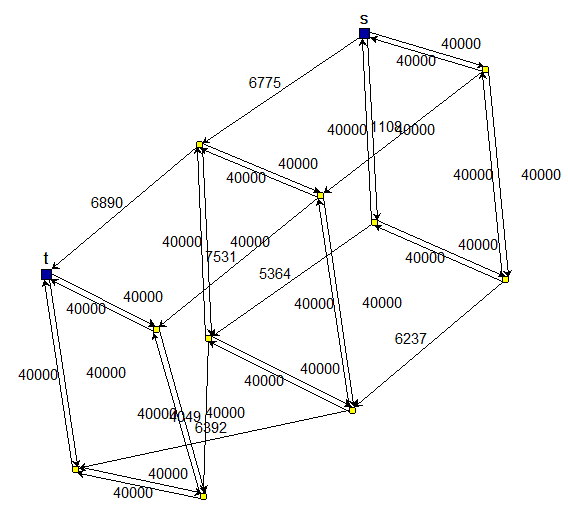
\includegraphics[width=90mm]{genrmf.png}
\caption{An example of the output of the GENRMF generator, where $a=2$ and $b=3$.}
\label{genrmfExample}
\end{figure}

The capacities between layers are randomly generated in the range $[c_{min}, c_{max}]$. 
Capacities inside layers are big enough so that all flow can be pushed around inside the layer.
This means we will have $n=a^2b$ nodes, and $m=4a(a-1)b + a(b-1)$ edges, which results in a relatively sparse graph.
As a consequence of the construction, the min-cut will always be between two layers.

We will use the generator in three modes, one which is long, where $a^2=b$, one which is flat, where $a = b^2$, and one which is square where $a=b$.


\subsection{Washington}
The Washington library is a collection of graph generators from DIMACS. We will use it to produce random level graphs.
The random level graph is a graph where the nodes are laid out in rows and columns. Each node in a specific row has edges to three random nodes in the following row.
The source has edges to all nodes in the first row, and all nodes in the last row has edges to the target.

We will use this to create two versions of the Wash graphs. A wide set of graphs that all have a constant 64 rows and a variable number of columns, and a long set of graphs with a constant 64 columns and a variable number of rows.


\begin{figure}[!ht]
\centering
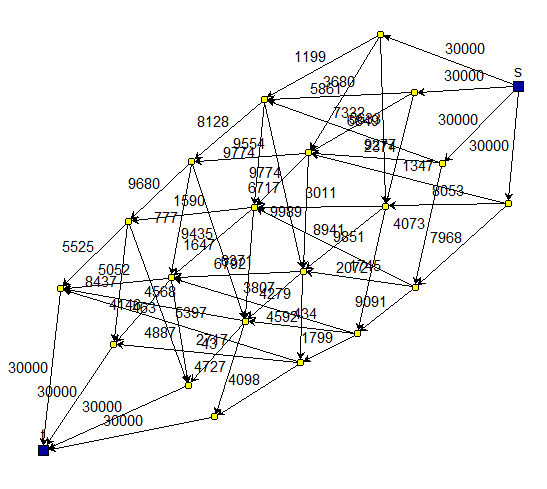
\includegraphics[width=90mm]{wash.png}
\caption{An example of the output of the washington level graph generator, with $5$ rows and $4$ columns}
\label{washExample}
\end{figure}

\clearpage
\subsection{Test Environment}
All tests were run on a Windows 7 64 bit PC with the hardware specified in Table~\ref{HardwareTable}.\\

\begin{table}[ht]
\begin{tabular}{ l r }
\hline
Processor & Intel Core I7 950 \\
Speed & 3.07 GHz \\
Cores & 4 physical, 8 logical\\
L1 Cache (Instruction) & 32 KB 4-way associative \\
L1 Cache (Data) & 32 KB 4-way associative \\
L2 Cache & 256 KB 8-way associative \\
L3 Cache & 8 MB 16-way associative (shared) \\
Cache Line & 64 bytes \\
\hline
Main Memory & Corsair CMZ12GX3M3A1600C9 \\
Capacity & 12 GB (3x4GB) \\
Speed & DDR3 1600 (PC3 12800) \\
Latency & CAS9 \\
\hline
\end{tabular}
\caption{Hardware specifications}
\label{HardwareTable}
\end{table}


